\section{问题介绍}

FAST项目目前能够观测到的信号范围为70 MHz到3 GHz,后期的工程目的是达到8GHz。为了实现更高频率的信号观测,需要提升馈源支撑系统的跟踪精度;为了提高终端系统的精度,需要考虑馈源支撑系统本身的自重等带来的反作用力。因此本文针对柔性支撑的并联机构,建立一个结构略不同于FAST项目馈源支撑系统的模型,从而放大支链反作用力因素,研究在给定外部干扰输入幅值和频率的情况下,通过设计控制器来抑制终端振动。

设计的系统运动学模型如图\ref{fig:kinetic_model}所示。基本的符号约定如下,
$A$代表世界坐标系;$B$代表Stewart\\
平台基座动平台所固结的坐标系,是扰动施加的位置;$C$代表Stewart静平台终端所固结的坐标系,是期望控制保持稳定的位置。此外,每个坐标系的中心均用$O_i$表示,比如$A$坐标系中心使用$O_A$表示。每条支链的长度使用$l_i$表示,$i$的值域为$\left\{ 1,2,3,4,5,6 \right\}$,代表6条支链序号。

\begin{figure}[H]
    \centering
    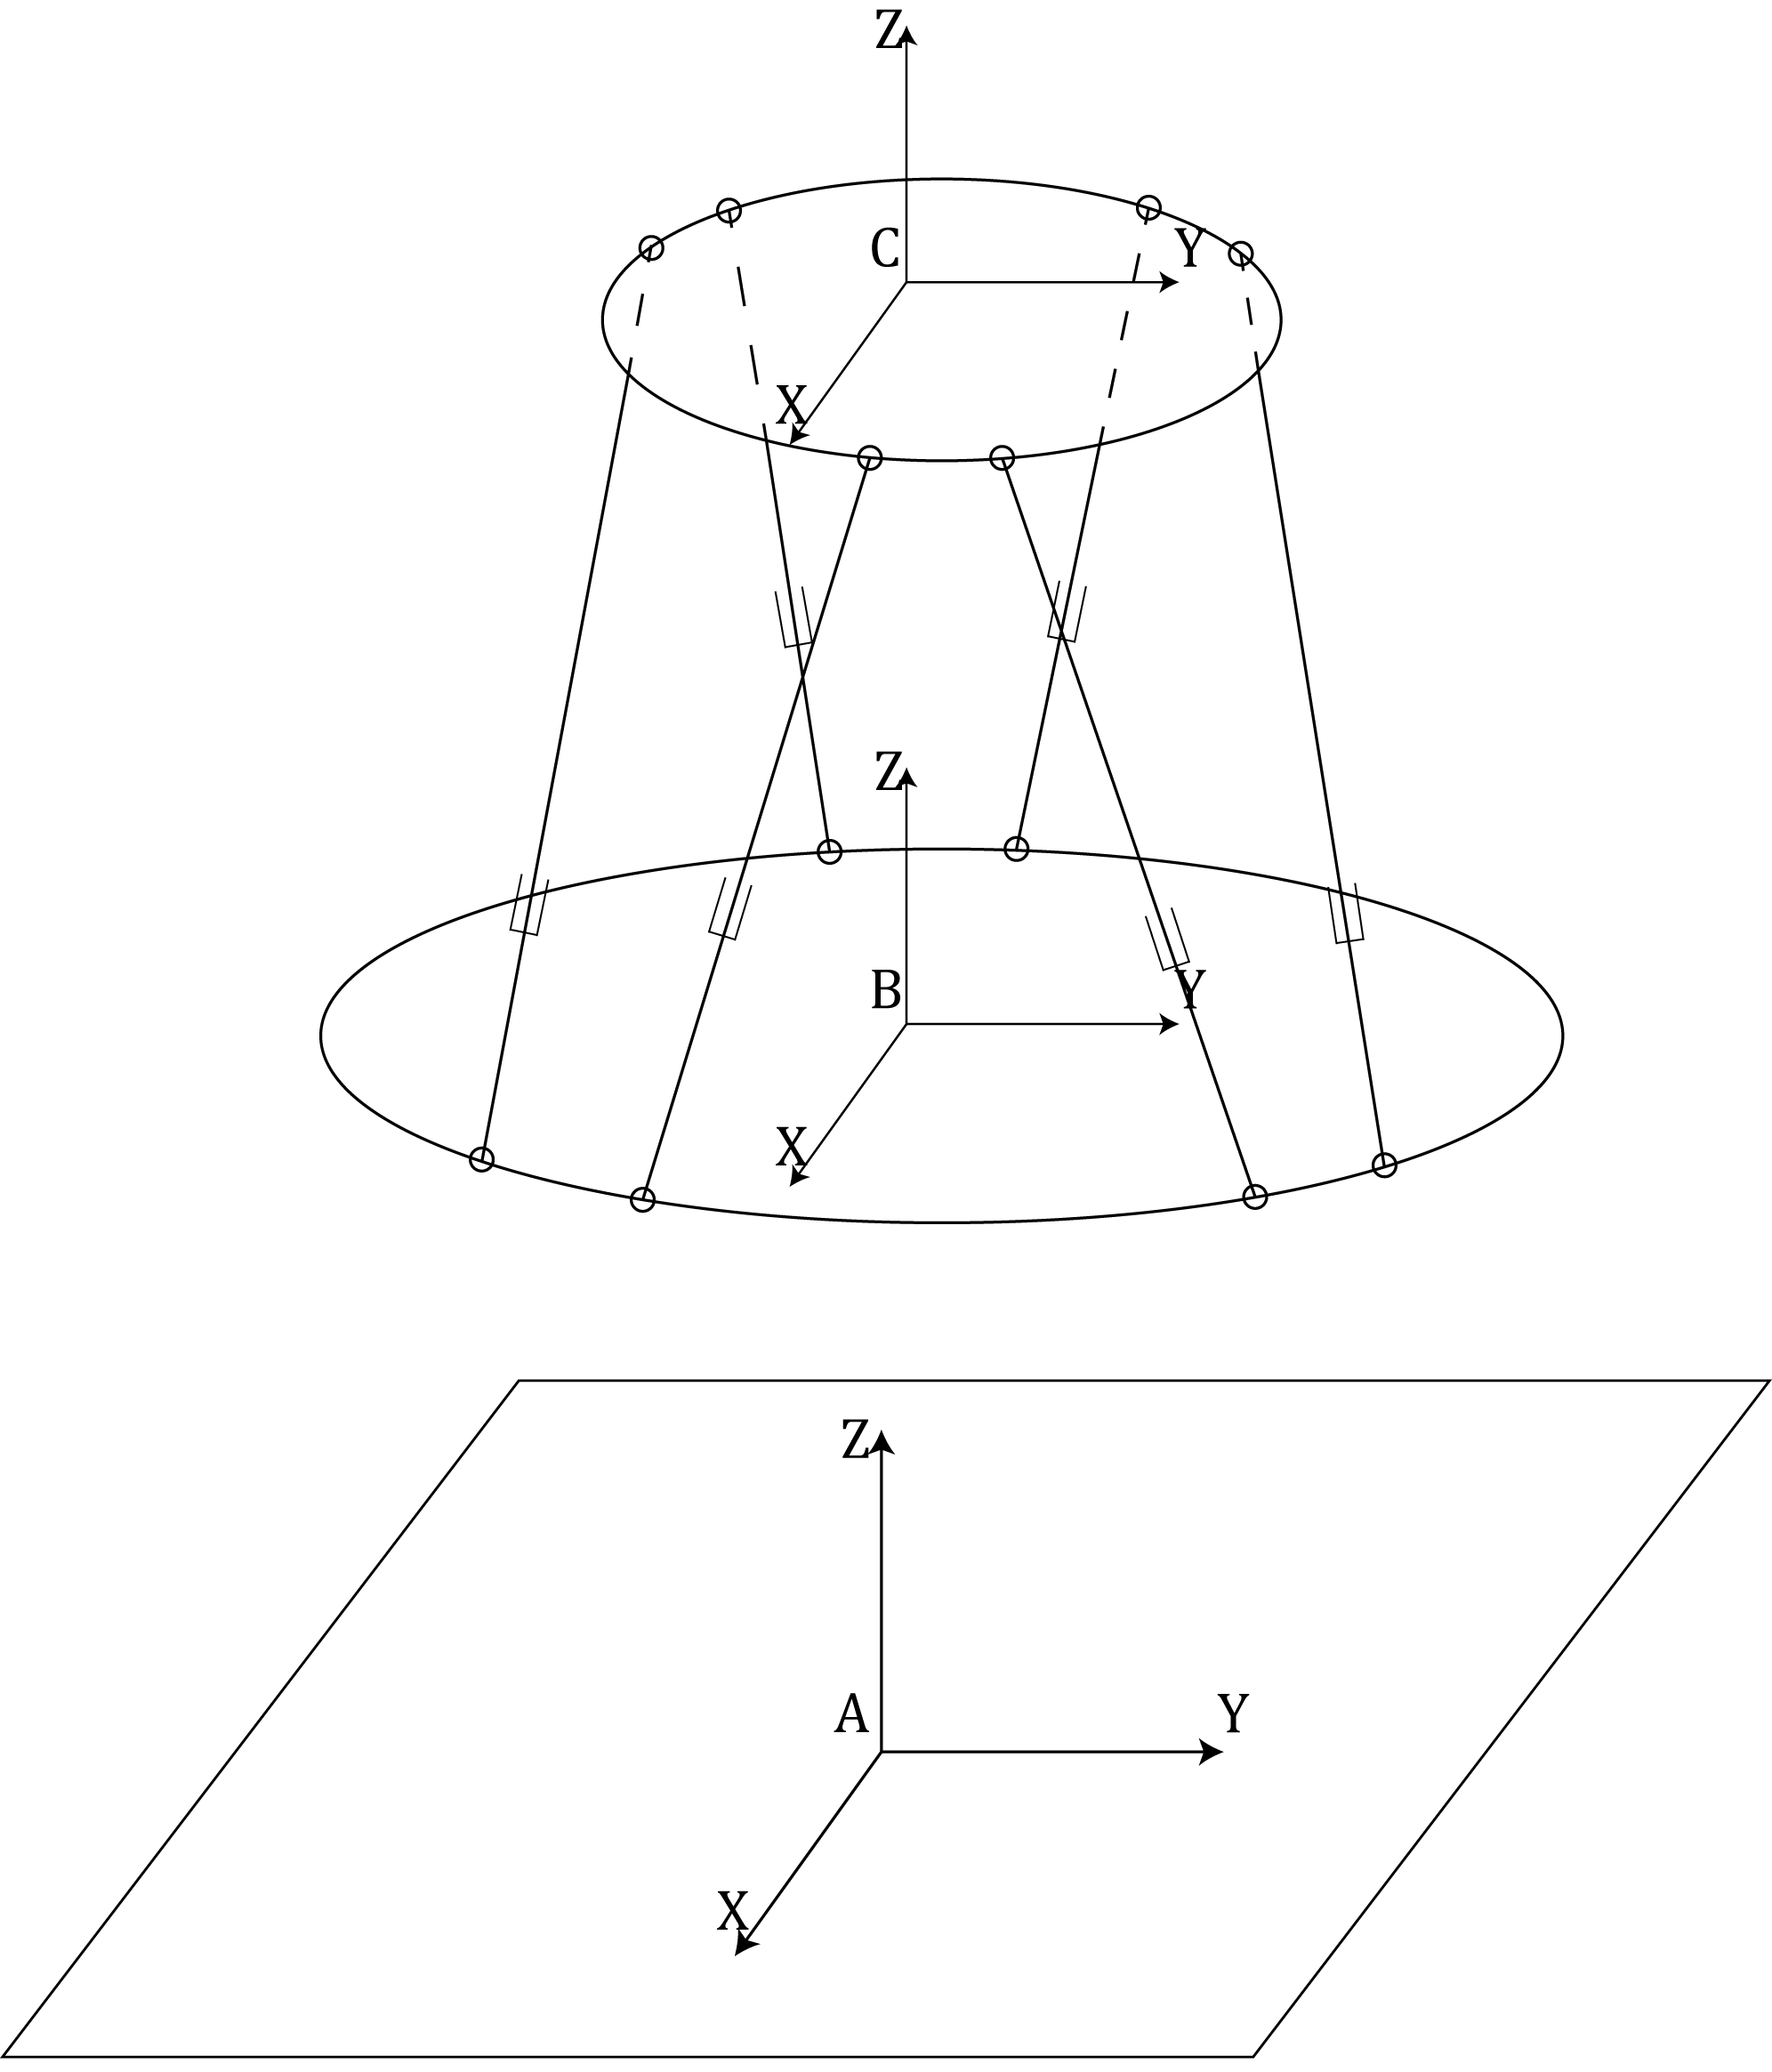
\includegraphics[width=0.4\textwidth]{./imgs/model_structure.png}
    \caption{运动学模型}
    \label{fig:kinetic_model}
\end{figure}

对于FAST本体,根据当地的气象观测数据,有史以来观测到的最大风力干扰为17 m/s,对馈源支撑系统的输入振动幅值为0.5 m\cite{nanFiveHundredMeter2006}。根据相应的有限元分析,支撑系统的前10阶模态为$ 0.004$ $\sim 0.18 \mathrm{Hz}$(另一机构结果为前18阶主频率为$0.15\sim 0.55\mathrm{Hz}$),表明需要注意到的振动输入频率主要为0.18Hz以下\cite{nanFiveHundredMeter2006}。对应于其50 m缩尺模型,指定的振动输入为幅值40 mm,频率$ 0.02 \sim 0.18 \mathrm{Hz}$,得到的最终闭环幅值控制精度为$ 15\sim 20 \mathrm{mm}$\cite{duanRouXingZhiChengStewartPingTaiDeFenXiYouHuaYuKongZhiYanJiu2008}。结合设计的这两个实验范围,本文装置的输入幅值最大为20 mm,输入频率保持为$ 0.02\sim 0.18 \mathrm{Hz}$。对于精度评价指标,闭环的幅值控制精度对应缩尺到$ 7.5\sim 10 \mathrm{mm}$。

% 可以发现,待控制的柔性支撑的Stewart平台,其具有非线性时变的特征,难以对其进行准确的建模和分析。因此具体来说,需要完成的控制器要满足下面几个特征:

% \begin{enumerate}
%     \item 控制器是基于无模型的控制
%     \item 控制器对噪声鲁棒,抗干扰能力强
%     \item 控制器输出受限,保证仪器安全
%     \item 控制器收敛速度快
% \end{enumerate}
\FloatBarrier
